\begin{figure*}[tp]
	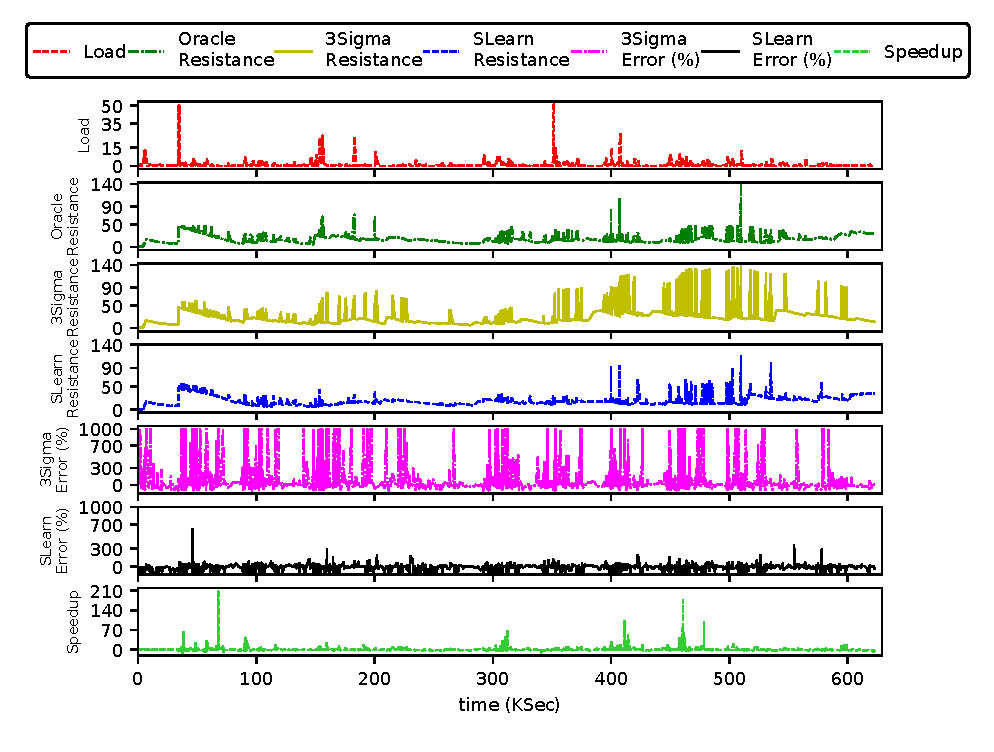
\includegraphics[width=1.0\linewidth]{figures/simulation/2STrace-Trial.eps}
	\caption{Correlation between load, \textit{resistance}, estimation error and speedup for 2STrace. \updated{16th Sep 2020}}
	\label{figs:sim:intuitionSpeedup:allInOne}
\end{figure*}


\section*{Appendix: Intuitive Explanation of Speedups}
\label{sec:sim:intuitionSpeedup}

% \S\ref{sec:sim:numPilots} - \S\ref{sec:sim:averageJCT} explain better
% performance under \slearn over \primarybase by experimental results.
In this section, we provide an intuitive explanation for \slearn's
improvement over \primarybasepredict.
Figure~\ref{figs:sim:intuitionSpeedup:allInOne} shows seven timeline
values comparing \slearn and \primarybase for the 2STrace as follows:

\begin{itemize}
\item The top curve shows the total workload arrived in the past 1000
  seconds, in terms of execution duration, for the 2STrace. The values
  are plotted in steps of 1000 seconds along the x-axis.  A unit along
  the y-axis corresponds to the workload that needs 1000 seconds
  of the entire cluster's compute capacity.
\item The next three curves show the \resistance faced by newly arrived jobs under
	\oracle, \primarybase and \slearn, respectively, where
	\resistance for a job is defined as the amount of higher
	priority workload existing at the time of its arrival
	{including} the remaining duration of the
	already scheduled tasks. A unit along the y-axis for these
	curves also corresponds to the workload that needs 1000
	seconds of the entire cluster's compute capacity. For wide
	jobs, under \slearn we show the value corresponding to the time
	when the job's size estimation is over and it has been placed
	in its estimated priority queue. \comment{The values are plotted along
	the x-axis corresponding to each job's arrival time.}
\item The next two curves correspond to the percentage error in
	\primarybasepredict and \slearn, respectively.  They show signed
	error which are capped at 1000, \eg a value of -20 on error
	curves means the job was estimated to be 20\% smaller and a
	value of 1000 means job was estimated at least 1000\%
	larger. The values are plotted along the x-axis corresponding
	to each job's arrival time.
\item The bottom curve shows the job speedup of \slearn over
	\primarybase.  Negative values mean the job slowed down under
	\slearn compared to \primarybase. The values are plotted along
	the x-axis corresponding to each job's arrival time.
        \comment{all values are above 1 or below -1???}
          
%	\questionaj{Should we also add speedup of \slearn vs. \oracle and
		%	\primarybase vs. \oracle. If yes, should we then move
		%	the \primarybase vs. \slearn speedup curve.}
\end{itemize}

With the above definitions of the curves, we next discuss what these curves
demonstrate intuitively.  The values on the \resistance curve indicate the
amount of workload which will be scheduled before the arriving job gets to run.
So, a job's completion time is roughly proportional to the \resistance it sees
upon arrival.  The \resistance, in turn, depends on the recently arrived
workload and the prediction error. If more workload has
arrived in the recent past, it is likely that
a newly arrived job will face higher \resistance.  More importantly, when the job is
estimated larger than its usual size, it may be misplaced in a lower priority
queue. If the error is more than 1000\% then the job will definitely be placed
in a lower priority queue. In such cases, the job will likely face higher
\resistance than it would have with accurate estimation.  Also, the jobs which
are underestimated may get placed in a higher priority queue. Though these jobs
will finish faster themselves but will create more \resistance for many other
jobs which are smaller than it and will slow them down. Only this part is hard
to visualize from the curves, but the other intuitions are easy to visualize
from the plots in figure \ref{figs:sim:intuitionSpeedup:allInOne}.  We can see
that the \resistance under \slearn is very similar to \oracle however under
\primarybase it is not.  Also, it is clearly visible that the peaks on
\resistance curve for \primarybase are mostly at the points where there is high
positive prediction error under \primarybase too.  Next, we can also see that
where there is higher \resistance  under \primarybase as compared to the
\slearn, those are the points where most of the peaks in the curve showing
speedup of \slearn over \primarybase are also observed.

%The data shown in table \ref{table:sim:overestimatedJobs} and
%\ref{table:sim:underestimatedJobs} also establishes the intuitive observations
%made from the curves.  \primarybase overestimates 59.37\% of the total jobs.
%Among the overestimated jobs, 36.02\% are misplaced at a lower priority queue,
%and among the misplaced jobs 82.84\% slowdown when compared to \oracle.
%Whereas \slearn overestimates 43.75\% of the total jobs. Among those only
%8.09\% are misplaced at a lower priority queue and are slowed down as compared
%to \oracle.
%%On the other side \primarybase underestimates 40.63\% of the jobs.
As visible from Fig.~\ref{figs:sim:intuitionSpeedup:allInOne}, most of the jobs
have low prediction error under \slearn whereas a significant number of jobs
have large prediction error under \primarybase. This explains why a larger
number of jobs, as shown in table \ref{table:sim:misplacedJobs:all}
%\ref{table:sim:overestimatedJobs} and \ref{table:sim:underestimatedJobs}, 
get misplaced under \primarybase and eventually deteriorate overall
performance.

%\questionaj{The current values in table \ref{table:sim:overestimatedJobs} and
%\ref{table:sim:underestimatedJobs} for \slearn are only for wide jobs and for
%\primarybase they are for all the jobs. What should we be doing here?}

\begin{table*}
\caption{Fraction of overestimated jobs and incorrect queue placement for 2STrace. Job performance in the third and seventh column is relative to the \oracle. \updated{2S - 16th Sep 2020}}
  \label{table:sim:misplacedJobs:all}
\vspace{-0.1in}	
  \centering
      {\small
	\begin{tabular}{|c|c|c|c|c|c|c|c|c|} 
	  \hline
		& Overestim- & Misplaced over- & Slowed mis- & Average (P50) & Underesti- & Misplaced under & Spedup mis- & Average (P50)\\
		& ated jobs & estimated jobs & placed jobs & Positive error & mated jobs & estimated jobs & placed jobs & Negative error\\
	  \hline
		%\primarybase & 59.37\% & 21.09\% & 17.72\% & 1253.60 (66.38)\% & 40.63\% & 10.22\% & 8.46\% & -39.33 (-31.59)\%\\
		\primarybase & 59.78\% & 17.50\% & 12.19\% & 898.45 (48.00)\% & 40.22\% & 8.65\% & 6.88\% & -37.0 (-28.57)\%\\
	  \hline
	  	\slearn & 43.75\% & 3.54 \% & 2.85\% & 30.65 (18.19)\% & 55.45\% & 7.37\% & 3.64\% & -26.79 (-20.69)\% \\
	  \hline
	\end{tabular}
      }
\vspace{-0.1in}	
\end{table*}

%\questionaj{I can add more numbers in the above line \eg jobs placed in a lower PQ but still performing better. Or jobs place in right queue but performing poor and similar number for jobs which were under estimated. But I think those will make things clumsy, please let me know what do you think?}
%maybe not 

In conclusion, whether a job finishes faster under \slearn compared to
\primarybase is a function of the prediction error. Due to high prediction
error in \primarybase, jobs get ordered incorrectly and hence face higher
\resistance, which results in longer finishing time under \primarybase.

%By looking at the 3Sigma resistance and error it becomes very evident that jobs
%which are estimated atleast 10$\times$ larger face much higher resistance as
%compared to what is observed for them in Oracle. This is because when estimated
%atleast 10$\times$ larger, the job will be moved to atleast 1 hop lower priority
%queue than it's actual queue. Since these queues are FIFO so all the workload of 
%the lower priority queue also adds to the resistance faced by the arriving job.
%In our experiments with the 2STrace \primarybase estimates 8(14)\% wide jobs 10(2-10) 
%$\times$ larger and all(half) of them are placed in a lower priority queue and
%more then 75(65)\% of them are slowed down compared to \slearn.
%
%No jobs in \slearn are estimated 10$\times$ or more larger.

